\chapter{讨论}
在这一章中我们对 \ref{chap-lenest} 中通过 RNA-Seq 数据估计转录本的长度的方法, 
\ref{chap-rna-seq-nonunif} 中对于 RNA-Seq 数据分布的不均匀性的描述, 
\ref{chap-rna-seq-nonunif} 中真核生物 RNA-Seq 数据估计基因的转录组问题是 NP 难的阐述, 
以及现有的 RNA-Seq 数据分析方法, 
和 RNA-Seq 数据分析方法的未来的发展方向进行讨论. 

\section{通过 RNA-Seq 数据估计转录本的长度}
在 \ref{chap-lenest} 的分析中我们只对单端等长读段测序数据进行了考虑, 
对于双端数据或者长度不均的读段均未作具体分析. 
在实际应用中可以只对双端数据考虑等长的在原转录本的 5' (或者 3') 端, 
或者长度不均的读段考虑等长的在原转录本的 5' (或者 3') 端, 
从而可以用 \ref{chap-lenest} 中的方法进行分析. 

此外, \ref{chap-lenest} 中所介绍的方法并没有考虑 RNA-Seq 
数据中读段分布受转录本序列以及转录本长度等因素造成的分布不均匀性. 
另外, \ref{chap-lenest} 中所介绍的方法也未考虑读段分布的非独立性. 
这些问题都是需要进一步继续的研究来解决的. 

\section{通过 RNA-Seq 数据估计基因的转录组}

\section{现有 RNA-Seq 数据处理方法中存在的一些问题}
目前已有的用于 RNA-Seq 数据辨识基因的剪切异构体和估计表达量的方法 
(\ref{intro-rna-seq-tools-summary}) 仍然存在不足. 
其中包括: 
\begin{itemize}
\item 辨识基因的剪切异构体复杂度高 (真核生物 RNA-Seq 数据)

\item 当有两个转录本其中一个转录本的一端位于另一个转录本的中间时 
(图 \ref{disc-human-gene-alternative-start-1}), 
目前没有有效的方法通过 RNA-Seq 数据对这两个转录本进行区分

\item 对于原核生物, 尤其是原核生物中的操纵子, 的分析方法仍然没有较规范的分析方法 
\cite{mcclure2013computational} (图 \ref{disc-bacteria-operons-1})

\item 估计转录本表达量时仍无系统的方法处理 RNA-Seq 数据中读段分布的不均性, 
以及转录本序列的组成带来的误差 \cite{oshlack2009transcript, jones2012new} 
\end{itemize}

\begin{figure}[!t]
\centering
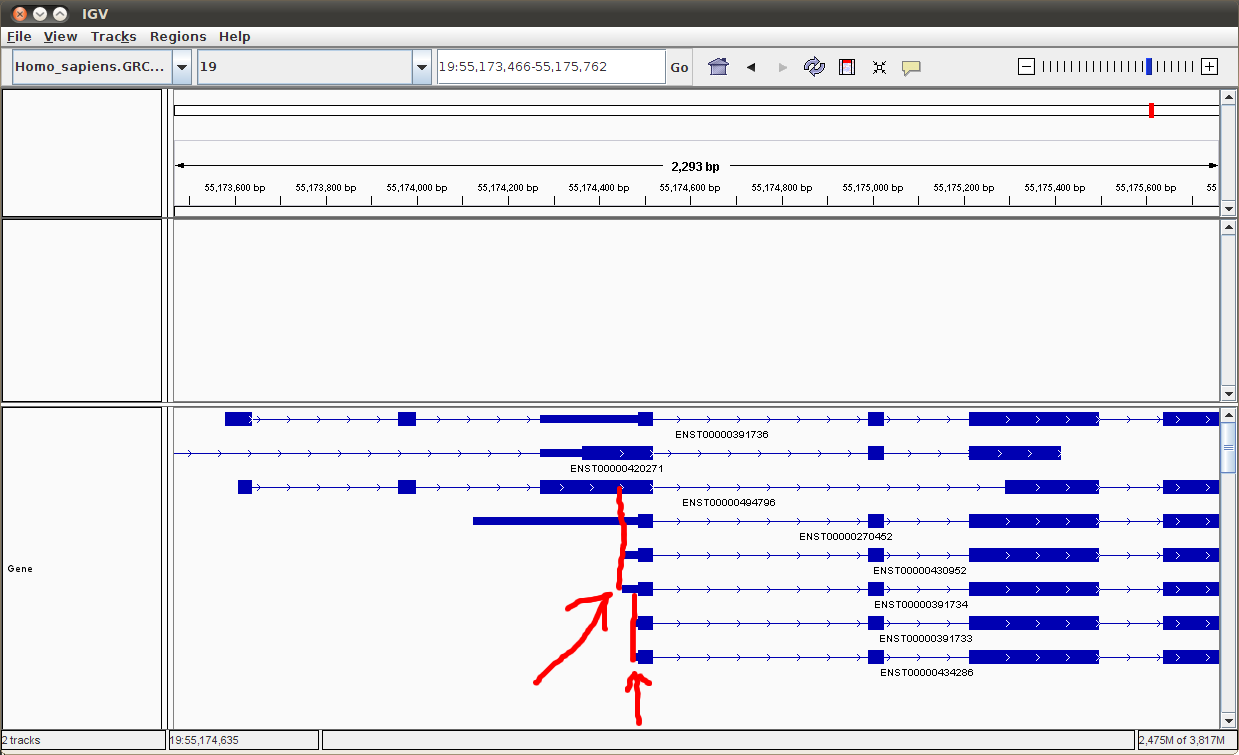
\includegraphics[width=\textwidth]{figures/disc/disc-human-gene-alternative-start-1.png}
\caption{人的基因组中出现的一个转录本的一端位于另一个转录本的中间的现象}
\label{disc-human-gene-alternative-start-1}
\end{figure}

\begin{figure}[!t]
\centering
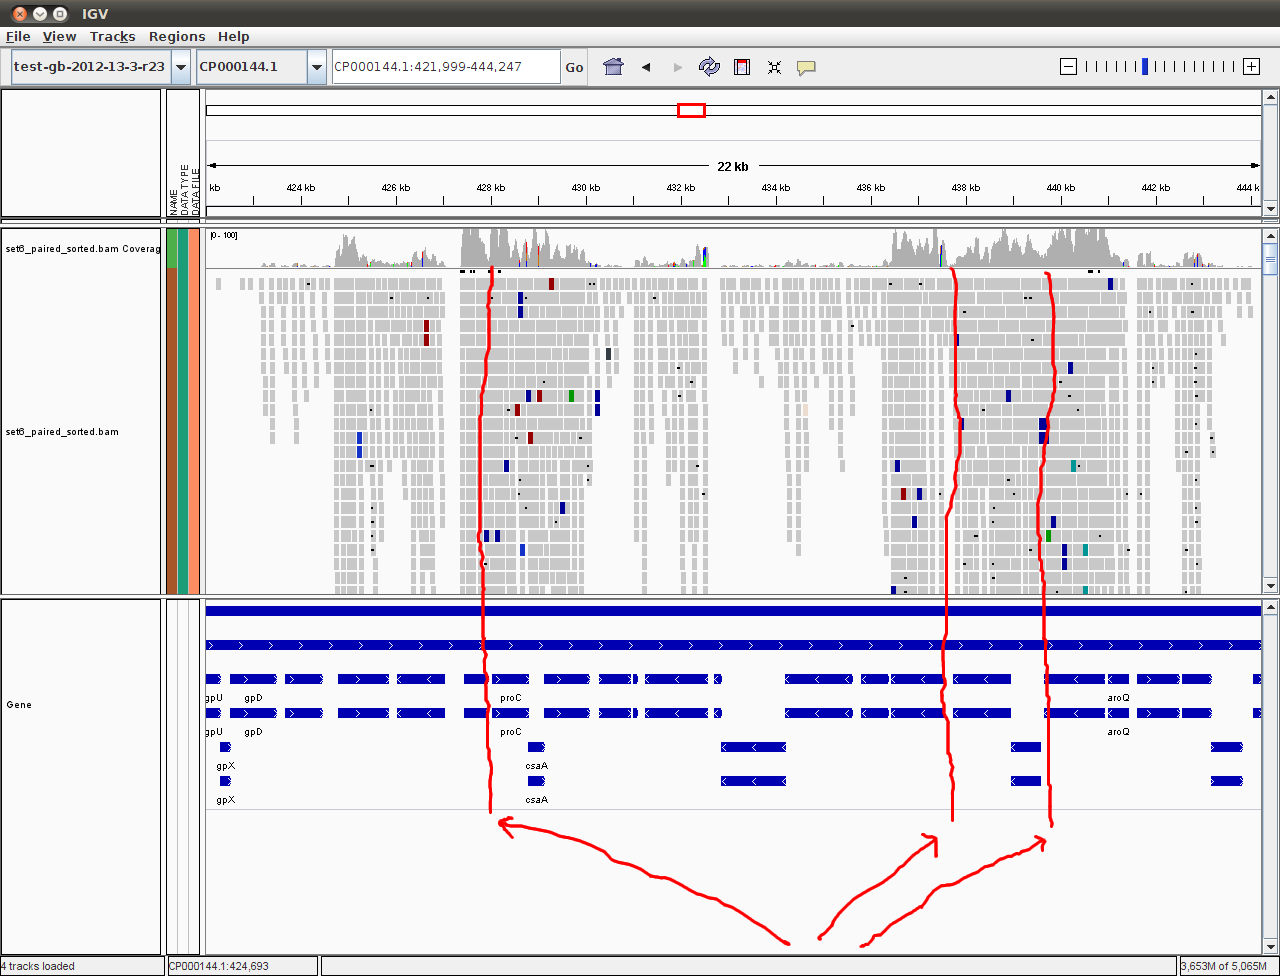
\includegraphics[width=\textwidth]{figures/disc/disc-bacteria-operons-1.png}
\caption{\onlinecite{giannoukos2012efficient} 中的 RNA-Seq 数据, 
其中可以看见多个基因构成的操纵子}
\label{disc-bacteria-operons-1}
\end{figure}

\section{未来 RNA-Seq 数据的定量分析方法的工作}

\subsection{真核生物}

\subsubsection{介绍} %% 需要测的读段更长

\subsubsection{RNA-PET 测序技术} %% 序列比对, 拼装

\subsubsection{PacBio 长读段} %% 序列比对, 拼装

\subsection{原核生物}

\subsubsection{介绍} %% 需要测的读段更长, 从 RNA-Seq 数据中分析操纵子
原核生物的 RNA-Seq 数据分析对于

\subsubsection{与真核生物 RNA-Seq 数据的比较} %% 计算上比原核生物更为简单, 模型相似
与真核生物不同, 原核生物中多个基因会被同时翻译到一个转录本中形成一个操纵子 
(图 \ref{e.coli.lactose.operon}).

\begin{figure}[!t]
\centering
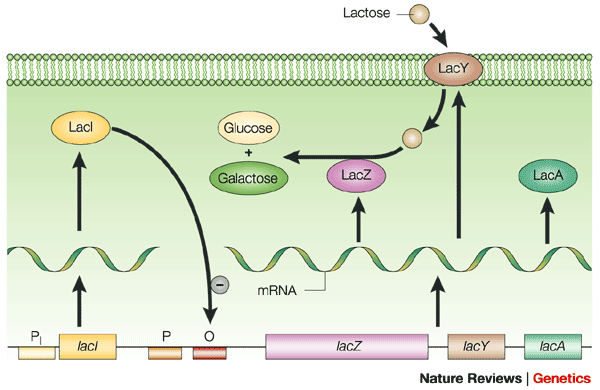
\includegraphics[width=\textwidth]{figures/disc/e-coli-lactose-operon.png}
\label{e.coli.lactose.operon}
\caption{\textit{E. coli} 中的乳糖操纵子 \cite{shuman2003art}}
\end{figure}

\subsubsection{RNA-PET 测序技术} %% 序列比对, 拼装





